%!TEX root = FreeRtos ARM uController.tex
\subsection{Scheduling}
\label{Scheduling}
Der Scheduler ist die Kernkomponente jedes Echtzeitbetriebssystem Kernels, da er eine quasi parallele Aus\-füh\-rung von Tasks ermöglicht. Eine Task stellt dabei ein ei\-gen\-stän\-di\-ge lauffähige Programmeinheit dar und wird ge\-wöhn\-lich in einer Schleife ausgeführt. Abhängig vom aktuellen Zustand der Tasks und dem gewählten Schedulingalgorithmus, wählt der Scheduler die nächste Task, die ausgeführt werden soll. Auf einem $\mu$\-Pro\-zesso\-r mit einem Kern kann dabei immer nur eine Task zur Zeit ausgeführt werden. Der Vorgang des Task-Wechsels durch den Scheduler wird Kontextwechsel oder Contextswitch genannt. Der Kontextwechsel beeinflusst nicht die Instruktionsfolge der Task. Zum Zeitpunkt der Unterbrechung wird durch den Scheduler eine Art Schnappschuss der Task erstellt, alle Register und der Stack der Task werden gesichert. Nachdem der Scheduler die verdrängte Task wieder zur Ausführung ausgewählt hat, werden alle Register und der Stack wieder hergestellt und in die entsprechenden $\mu$\-Pro\-zesso\-r Register geladen. Die Task wird danach ab der letzten Instruktion fortgeführt. Abbildung \ref{fig:ContextSwitch} zeigt wie eine Task während ihrer Ausführung unterbrochen wird.
\begin{figure}[ht!]
	\centering
		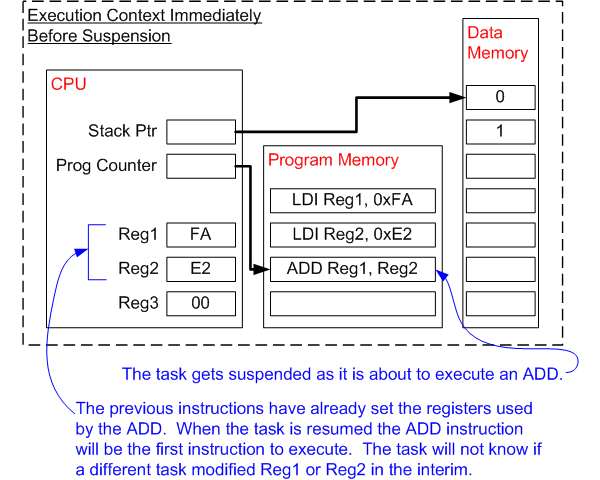
\includegraphics[width=0.4\textwidth]{Pictures/FreeRTOSOrg/ExeContext.png}
	\caption{Der Kontextwechsel einer Task findet mitten in der Ausführung statt. Alle Register die für die weitere Ausführung benötigt werden, werden durch den Scheduler gesichert. Bild-Quelle~\protect\citeA{MasteringFreeRtos} }
	\label{fig:ContextSwitch}
\end{figure}
\newline
Neben den User-Tasks, die durch den Entwickler erstellt werden, gibt es noch die Idle Task. Diese wird automatisch beim Start des Schedulers erstellt. Die Idle Task hat immer die niedrigste Priorität (0) und wird immer dann ausgeführt, wenn keine User-Task zur Ausführung bereit steht. Die Idle Task ist ein Indikator für über\-schüss\-ige Prozessorzeit. Mittels der Idle-Hook Funktion kann der Idle Task Funktionalität durch den Entwickler hinzugefügt werden. Wie die Idle Task zum Energiesparen genutzt werden kann, wird in Abschnitt \ref{sec:Low Power Modes} beschrieben.
\newline
\needspace{3\baselineskip}   
Folgende Zu\-stän\-de kann eine FreeRTOS Task im Scheduling annehmen: 
\begin{itemize}
	\item Running: Die Task wird zur Zeit vom Scheduler ausgeführt
	\item Blocked: Die Task ist nicht bereit und warten auf ein Synchronisations- oder ein Timer Event
	\item Ready: Die Task ist bereit und warten auf ihre Aus\-füh\-rung durch den Scheduler
	\item Suspended: Die Task hat vTaskSuspend() aufgerufen und wurde vom Schedulingvorgang ausgeschlossen
\end{itemize}
 Abbildung \ref{fig:TaskStates} zeigt ein vollständiges Zustandsdiagramm einer FreeRTOS Task.
\begin{figure}[ht!]
	\centering
		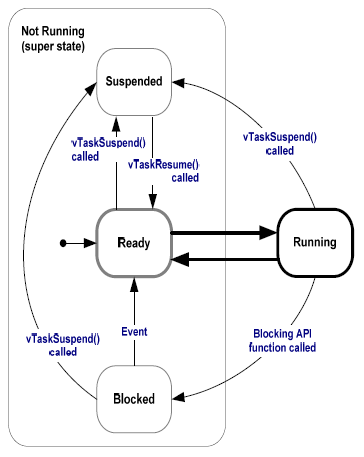
\includegraphics[width=0.2\textwidth]{Pictures/FreeRTOSOrg/taskStates.png}
	\caption{Übersicht aller Task Zustandstransitionen in FreeRTOS. Der Zustandswechsel findet entweder durch den Aufruf einer FreeRTOS API Funktion statt3oder aber durch Event z.B. Interrupts, Timer-Events. Der Wechsel in den Zustand Running wird durch den Scheduler bestimmt und ist durch den Schedulingalgorithmus definiert.  Bild-Quelle~\protect\citeA{MasteringFreeRtos}}
	\label{fig:TaskStates}
\end{figure} 
\newline
Die Grundlage aller zur Verfügung stehenden Schedulingalgorithmen, ist das Round Robin Verfahren\cite{9783827373427}. Dabei werden alle lauf\-fäh\-igen Tasks (Ready) gleicher Priorität in einer Liste verwaltet. Jede Task in der Liste erhält ein gewisses Zeitquantum\footnote{Round Robin definiert nicht die Länge des Zeitquantums}, welches bestimmt wie lange einer Task der Prozessor zugeteilt wird. Nach Ablauf des Zeitquantum wird ein Kontextwechsel durchgeführt und die näch\-ste Task in der Liste erhält Prozessorzeit. Die ausgelaufene Task wird durch den Scheduler automatisch hinten an die Liste angefügt. Da jeder Task in FreeRTOS eine gewisse Priorität zugewiesen wird, ist auch für jede Priorität eine eigene Round Robin-Liste nötig. Dieses Verfahren wird auch Priority Scheduling \cite{9783827373427} genannt. Abbildung \ref{fig:PrioList1} veranschaulicht den Aufbau dieser Listen und in Listing \ref{lst:nextTask} wird gezeigt wie das Priority Scheduling im FreeRTOS Source Code umgesetzt wurde. 
\begin{figure}[ht!]
	\centering
		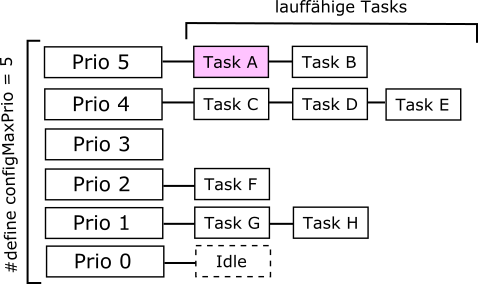
\includegraphics[width=0.3\textwidth]{Pictures/Scheduling/PrioList1.png}
	\caption{Aufbau der Prioritätenliste nach Round Robin in FreeRTOS. Alle aufgeführten Task sind bereit zur Ausführung. Task A wird aktuell durch den Scheduler ausgeführt. Nach dem Ablauf des Zeitquantums, wird A hinter B einsortiert. Die Maximale Priorität wird durch configMaxPrio bestimmt. Die Idle Task wird automatisch durch den Kernel erzeugt und hat immer die niedrigste Priorität. }
	\label{fig:PrioList1}
\end{figure}
\begin{lstlisting}[caption={FreeRTOS Source zur Priroty Task Selection aus Task.c. Alle lauffähigen Task werden in einem Array vewaltet pxReadyTaskLists. Die Listen verwalten sich durch Referenz-Pointer in den TCBs der einzelnen Tasks}, linewidth=8cm,captionpos=b, label=lst:nextTask, float=hbt]
#define taskSELECT_HIGHEST_PRIORITY_TASK(){																									
	UBaseType_t uxTopPriority = uxTopReadyPriority;														
		/* Find the highest priority queue that contains ready tasks. */								
		while(listLIST_IS_EMPTY(&(pxReadyTasksLists[ uxTopPriority ]))){																								
			configASSERT( uxTopPriority );																
			--uxTopPriority;																			
		}																								
		/* listGET_OWNER_OF_NEXT_ENTRY indexes through the list, so the tasks of						
		the	same priority get an equal share of the processor time. */									
		listGET_OWNER_OF_NEXT_ENTRY(pxCurrentTCB, &(pxReadyTasksLists[uxTopPriority]));			
		uxTopReadyPriority = uxTopPriority;																
	} /* taskSELECT_HIGHEST_PRIORITY_TASK */
\end{lstlisting}
\newline
\newline
Dem Entwickler stehen zwei Konfigurationsmöglichkeiten des FreeRTOS Scheduler zur Auswahl. Der Scheduler kann entweder im Cooperative Modus oder im Preemptive Modus ausgeführt werden. Welcher Modus vom Scheduler als Schedulingalgorithmus verwendet wird, wird durch das folgende define in der FreeRTOS config bestimmt.
\begin{lstlisting}[numbers = none]
#define configUSE_PREEMPTION
\end{lstlisting}
Im Preemptive Modus wird eine aktive Task mit niedriger Priorität sofort von einer Task mit höherer Priorität verdrängt und ein Kontextwechsel wird durchgeführte. Im kooperativen Modus hingegen wird ein Kontextwechsel erst durchgeführt, wenn eine Task den Prozessor explizit durch die Funktion xTaskYield() abgibt. Abbildung \ref{fig:PreVSCo} zeigt den Vergleich beider Modis durch einen beispielhaften Ablauf. 
\begin{figure}[htb]
	\centering
		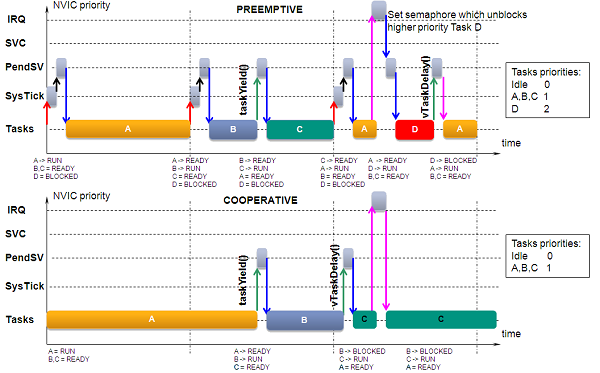
\includegraphics[width=0.5\textwidth]{Pictures/EMCUIT/PreemptiveCooperative.png}
	\caption{Im Co-operative Modus wird der Prozessor von einer Task erst abgegeben, wenn diese explizit taskYield() aufruft. Selbst wenn eine Task mit höhrer Priorität in den Ready Zustand wechselt, läuft die Task mit niedrigerer Priorität weiter. Im Gegensatz dazu steht das Pre-Emptive Scheduling (hier mit Time-Slicing), es unterbricht die laufende Task mit niedriger Priorität sofort, sobald eine Task mit höherer Priorität Ready ist. Bild-Quelle~\protect\citeA{MasteringFreeRtos}}
	\label{fig:PreVSCo}
\end{figure}
Für den Preemptive Modus bietet FreeRTOS eine weitere Konfigurationsmöglichkeit. \needspace{3\baselineskip}Mit der nachfolgenden Pre-Prozessordirektive lässt sich ein Zeitschlitzverfahren (time slicing) aktivieren. 
\begin{lstlisting}[numbers = none]
#define configUSE_TIME_SLICING 1
\end{lstlisting}
Durch das Zeitschlitzverfahren wird die zugeteilte Prozessorzeit für Task gleicher Priorität gleichmäßig aufgeteilt. Dies geschieht durch Ein\-füh\-rung eines festen Tick-Interrupt Intervalls. Bei jedem Tick Interrupt wird der FreeRTOS SysTickHandler aufgerufen. Listing \ref{lst:SysTickS} zeigt die Implementierung des FreeRTOS SysTicks. Der SysTickHandler ist Bestandteil des Schedulers und überprüft bei jeder Ausführung, ob sich eine Task gleicher Priorität im Ready Zustand befindet. Sollte es eine solche Task geben wird ein Kontextwechsel durchgeführt und die Task erhält den Prozessor zugeteilt. Des Weiteren kümmert sich der SysTickHandler um die Verwaltung des TickCount, welcher als Referenz für alle RTOS Timingfunktionen dient. Abbildung \ref{fig:SysTick} zeigt diesen Vorgang nochmal im zeitlichen Verlauf. 
\begin{lstlisting}[caption={FreeRTOS Source des SysTickHandlers aus Task.c. Der SysTickHandler verwaltet den TickCount. Der TickCount dient allen Timingfunktionen des RTOS Kernels als Zeitreferenz. Des Weiteren wird bei aktivem Time Slicing überprüft ob ein Kontextwechsel nötig ist. Der Kontext wechsel wir dann ggf. durch den PendSVHandler durchgeführt.}, linewidth=8cm,captionpos=b, label=lst:SysTickS, float=hbt]
void xPortSysTickHandler( void ){
	portDISABLE_INTERRUPTS();
	{
		/* Increment the RTOS tick. */
		if( xTaskIncrementTick() != pdFALSE )
		{
			/* A context switch is required.  Context switching is performed in
			the PendSV interrupt.  Pend the PendSV interrupt. */
			portNVIC_INT_CTRL_REG = portNVIC_PENDSVSET_BIT;
		}
	}
	portENABLE_INTERRUPTS();
}
\end{lstlisting}
\begin{figure}[htb]
	\centering
		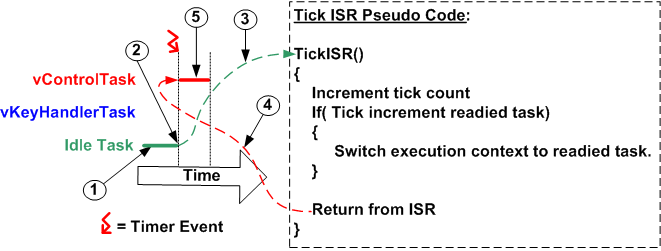
\includegraphics[width=0.4\textwidth]{Pictures/FreeRTOSOrg/TickISR.png}
	\caption{Beispielhafter Ablauf eines SysTickInterrupts.(1) keine User Task ist ready, die Idle Task ist aktiv. (2) SysTickInterrupt. (3) SysTickHandler wird aufgerufen. (4) vControlTask ist ready und ein Kontext wechsel wird durchgeführt. vControlTask hat hier die gleiche Priorität wie die IdleTask. (5)vControlTask wird ausgeführt. Bild-Quelle~\protect\citeA{MasteringFreeRtos}}
	\label{fig:SysTick}
\end{figure}
\newline
Die wohl am häufigsten verwendete Konfiguration ist der Preemptive Modus mit aktivem Zeitschlitzverfahren.
\begin{lstlisting}[numbers = none]
#define configUSE_PREEMPTION 1
#define configUSE_TIME_SLICING 1
\end{lstlisting}
Diese Einstellung wird üblicherweise Prioritized Pre-emptive Scheduling with Time Slicing genannt. Abbildung \ref{fig:timeslice} zeigt wie sich diese Konfiguration des Schedulers bei mehreren Task mit unterschiedlicher Priorität verhält.
\begin{figure}[htb]
	\centering
		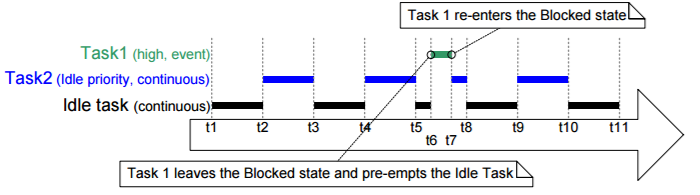
\includegraphics[width=0.5\textwidth]{Pictures/Scheduling/timeslice2.png}
	\caption{Durch das Zeitschlitzverfahren wechseln sich Task1 und Idle Task bei jedem SysTick Interrupt ab, da beide die gleiche Priorität haben. Bei T6 ist Task 1 bereit und verdrängt (preempt) aufgrund ihrer höheren Priorität Task2. Nachdem Task 1 blockiert, wird Task 2 fortgeführt. Bild-Quelle~\protect\citeA{MasteringFreeRtos}}
	\label{fig:timeslice}
\end{figure}







